\section{More-sophisticated behavior}

\subsection{Selfstudy-Questions OOP6}

\subsubsection{Chapter 5.2 - The TechSupport system}

\subsubsection*{Exercise 1}
\textit{Solve the exercise 5.1}\\

\lstinputlisting{../workspace/TechSupport/src/support/Main.java}

\subsubsection*{Exercise 2}
\textit{At page 157 and 158 there is a Method start() that uses a 
while-loop. Create a code snippet with the same functionality by using a
do-while loop.}\\

\begin{lstlisting}
public void start()
{
	boolean finished = false;

	printWelcome();

	do{
		String input = reader.getInput();
		if(input.startsWith("bye")){
			finished = true;
		} else{
			String response = responder.generateResponse();
			System.out.println(response);
		}
	}while(!finished)
	
	printGoodbye();
}
\end{lstlisting}

\subsubsection{Chapter 5.3 - Reading class documentation}

\subsubsection*{Exercise 3}
\textit{Solve the exercises 5.2 to 5.5 as well as 5.7 to 5.11}\\

\textbf{5.2} The Java documentation has a clear design. Every class like 
String is described in different sections, to get as fast as possible to the
information needed. This documentation is arranged by the following 
sections:

\begin{itemize}
	\item Summary
	\begin{itemize}
		\item Nested
		\item Field
		\item Constructor
		\item Method
	\end{itemize}
	\item Detail
	\begin{itemize}
		\item Field
		\item Constructor
		\item Method
	\end{itemize}
\end{itemize}

\textbf{5.3} The class String has two methods called startsWith, where
one method has only one parameter (String) and the other has two parameters
(String and int).
The method that has only one parameter is returning \lstinline{true} if the
specified string is found at the very beginning of the specified String
object.
The other method with two parameters is returning \lstinline{true} if the
specified string is found after the specified offset. The offest is a
int value representing the number of characters.

Here is an example for the behavior. Both of these \lstinline{if} statements
are returning \lstinline{true}.

\begin{lstlisting}
String s = "Hi, my name is Avaj Elcaro.";

// check if the very beginning of the String object is "Hi"
if(s.startsWith("Hi")){
	System.out.println("found match at the very beginning");
}

// check if the String object has the string "my" after the 4th character
if(s.startsWith("my", 4)){
	System.out.println("found match after the 4th character");
\end{lstlisting}

\textbf{5.4} There is a method in the class String that checks if a 
String ends with a specified suffix.

\begin{lstlisting}
public boolean endsWith(String suffix)
\end{lstlisting}

\textbf{5.5} There is a method in the class String that returns the number
of unicode characters in a specified string.

\begin{lstlisting}
public int length()
\end{lstlisting}

\subsubsection*{Exercise 4}
\textit{In which package do you suppose the class FileWriter?
Check your guess with the Java API documentation.}\\

The class FileWriter is a part of the package java.io where the io stands
for Input-Output.

\subsubsection*{Exercise 5}
\textit{With the class BufferReader you can read files line by line.
How does that work? You can find the answer in the Java API documentation.}\\

We can use the method readLine() for that job. Here is an example form
\url{http://www.roseindia.net/java/beginners/java-read-file-line-by-line.shtml}

\begin{lstlisting}
import java.io.*;
class FileRead 
{
 	public static void main(String args[])
  	{
  		try{
  			// Open the file
			FileInputStream fstream = new FileInputStream("textfile.txt");
  			// Get the object of DataInputStream
  			DataInputStream in = new DataInputStream(fstream);
  			BufferedReader br = new BufferedReader(new InputStreamReader(in));
  			String strLine;
  			//Read File Line By Line
  			while ((strLine = br.readLine()) != null)   {
  				// Print the content on the console
				System.out.println (strLine);
  			}
  			//Close the input stream
  			in.close();
		}catch (Exception e){//Catch exception if any
			System.err.println("Error: " + e.getMessage());
  		}
	}
}
\end{lstlisting}

\subsubsection{Chapter 5.4 - Adding random behavior}

\subsubsection*{Exercise 6}
\textit{Solve the exercises 5.12 and 5.13}\\

\textbf{5.12} The Random class is from the package java.util. It is used to
generate a stream of pseudorandom numbers. An instance can be constructed
with the following code.

\begin{lstlisting}
import java.util.Random;

public class Main
{
	public static void main(String[] args)
	{
		// create an instance of Random
		Random rand = new Random();

		// print out 10 random numbers between 0 and 20
		for(int i = 0; i < 10; i++)
		{
			System.out.println(rand.nextInt(21));
		}
	}
}
\end{lstlisting}

\textbf{5.13} See 5.12

\subsubsection*{Exercise 7}
\textit{Solve the exercise 5.15}\\

If we use \lstinline{rand.nextInt(100)} we will get any integer number 
between 0 and 99.

\subsubsection*{Exercise 8}
\textit{Solve the exercise 5.18}\\

Simple example of a random response program.

\lstinputlisting{../workspace/Snippets/src/randomResponse/RandomResponse.java}

\subsubsection{Chapter 5.5 - Packages and import}

\subsubsection*{Exercise 9}
\textit{Solve the exercises 5.21 and 5.22}\\

\textbf{5.21} See Exercise 8 - 5.18

\textbf{5.22} If we implement the response generation like in the example code 
above, it will work for any number of responses in the ArrayList. This is 
because the code is flexible for the size of the ArrayList.

\newpage
\subsection{Selfstudy-Questions ALG1}

\subsubsection*{Exercise 10}
\textit{Describe in words or as pseudocode one algorithm per problem.}\\

\begin{enumerate}[label={(\alph*)}]
	\item \textit{Calculate the product of two integers without a 
		multiplication-operator.}\\

		One possible approach to solve this problem could be to
		use simple addition and iteration. This is because a 
		multiplication, for example $3 \cdot 5 = 15$, can be
		substituted with $(3 + 3 + 3 + 3 + 3) = (5 + 5 + 5) = 15$.
		\lstinputlisting{../workspace/Snippets/src/multiply/Multiplier.java}
		\lstinputlisting{../workspace/Snippets/src/multiply/Main.java}

		An alternative approach is to think of the factors as binary
		numbers. In the binary system we multiply also by a addition.
		See the following example: Lets multiply $11 \cdot 14 = 154$.
		In binary this looks like following:
		\[ \begin{array}{l r | l}
			& \texttt{1011}_b & 11_d \\
			\cdot & \textcolor{red}{1}
				\textcolor{green}{1}
				\textcolor{cyan}{1}
				\textcolor{blue}{0}_b & 14_d \\
			\hline \hline 
			& \texttt{0000}_b & \textcolor{blue}{0} \cdot 1011_b \\
			+ & \texttt{1011~}_b & \textcolor{cyan}{1} \cdot 1011_b \text{ and leftshift by 1} \\
			+ & \texttt{1011~~}_b & \textcolor{green}{1} \cdot 1011_b \text{ and leftshift by 2}\\
			+ & \texttt{1011~~~}_b & \textcolor{red}{1} \cdot 1011_b \text{ and leftshift by 3} \\
			\hline \hline
			= & \texttt{10011010}_b & 154_d
		\end{array} \]
		If we wanted to implement that alorithm, we would have to 
		operate binary, but in fact that would be not really 
		different form the fist approach.
	\item \textit{Find the lowest number out of a sequence like 
		$S = {4,-1,50,10,0,1,-2,5,10}$}\\
		
		\lstinputlisting{../workspace/Snippets/src/search/Main.java}
\end{enumerate}

\subsubsection*{Exercise 11}
\textit{Implement an algorithm to calculate the greatest common divisor
with the modulo operator (see ALG1 presentation, page 12).}\\

\lstinputlisting{../workspace/Snippets/src/euklid/Main.java}

\begin{enumerate}[label={(\alph*)}]
	\item Test your algorithm with some examples.
	\item Change your algorithm so that you don't use the modulo operator. 
		Change the modulo operation with a combined expression and test 
		your implementation again. \\
		\textit{Hint: The modulo operator can be substuituted by a 
			sequence of subtractions that is finished as the 
			result is smaller than the subtrahend.}
		\lstinputlisting{../workspace/Snippets/src/euklid2/Main.java}

\end{enumerate}

\subsubsection*{Exercise 12}
\textit{What's the order of the algorithm to calculate the n-th pseudo random 
number z (see OOP6 presentation page 28 and ALG1 presentation page 15)?}\\

\[ z_{n+1} = (a \cdot Z_n + r) \% m \]

\subsection{Programming Exercise}
\textit{Write a class FormLetter that is able to produce serial letters.
The class has an ArrayList of type FormalAddress (see OOP3). With the 
method addAddress() a new object of type FormalAddress is generated and
added to the ArrayList. With the method void print(int actualYear, String
subject, String textBody) a new serial letter is generated for all 
elements in the ArrayList. The letter contains a greeting, a subject and
of cource the text itself. This shall be printed to the console.}

\lstinputlisting{../workspace/FormLetter/src/letter/Main.java}
\lstinputlisting{../workspace/FormLetter/src/letter/FormLetter.java}
\lstinputlisting{../workspace/FormLetter/src/letter/FormalAddress.java}

\subsection{Team-Exercise}
\subsubsection{Exercise 1}
\textit{Create a class ListIteratorApplication with the attribute of type
ArrayList for Strings. Fill the ArrayList with the words of the sentence
"With the iterator it is possible to tavers Lists back and forth".
\begin{enumerate}
	\item Program a method iterateDown() that is iterating through 
	the ArrayList. Use a Iterator for this method.
	\item Program a method iterateUp() that is iterating reverse
		through the ArrayList. Use a for-loop and the get()
		method form ArrayList.
	\item Program a method iterateBothWays() that is iterating
		through the ArrayList and then backwards. Use the
		ListIterator for this method and take a look at the
		API documentation of it.
	\item Optional Ecerxice: Use the StringTokenizer to fill the 
		ArrayList. An example is given by the OOP5 presentation
		on page 10. Take also a look at the API documentation.
\end{enumerate}}

\lstinputlisting{../workspace/ListApp/src/list/Main.java}
\lstinputlisting{../workspace/ListApp/src/list/ListIteratorApplication.java}

\subsubsection{Exercise 2}
\textit{A sequence of integers is arranged in an array.
	A subsequence of a sequence is of arbitrary length but is combined
	by trailed parts of it. See the following example.} \\ \\
\lstinline!int[] series = {5, -8, 3, 4, -5, 7, -2, -7, 3, 5}! \\
\lstinline!int[] subseries1 = {5, -8, 3}! \\
\lstinline!int[] subseries2 = {-5, 7, -2, -7, 3}! \\ \\
\textit{Of course an empty sequence is also a valid subsequence.
A subtotal is the sum of all entries of a subsequence. The subtotal of
subseries1 form the example is 0, the subtotal of subseries2 is -4.
An empty subsequence has the subtotal 0.
The following pseudocode describes a intuitiv algorithm.}

\begin{lstlisting}
For all start values form 0 up to the length of the sequence
    For all end values from start value up to the length of the sequence
        Calculate the sum of the subsequence form start value up to the end value
        Is it the maximum sum?
\end{lstlisting}

\textit{
\begin{enumerate}
	\item What order has the algorithm described above?
	\item Create a method public int maxSubtotal(int[] sequence) in class
		Series, which implements the algorithm above.
	\item Test your implementation with a testmethod, which generates 
		different sequences and calls the method maxSubtotal().
\end{enumerate}
}



\subsection{Selfstudy-Questions OOP7}

\subsubsection{Chapter 5.6 - Using maps for associations}

\subsubsection*{Exercise 1}
\textit{Solve the exercises 5.24 to 5.30} \\

\textbf{5.24} HashMap is a parameterized class and these are
the mehtods that depend on the type.

\textbf{5.25} If we want to know how many entries are 
contained in a map we can use the \lstinline{size()} method.

\textbf{5.26} A very simple phone book implementation with HashMap.
\lstinputlisting{../workspace/Snippets/src/phoneBook/Main.java}
\lstinputlisting{../workspace/Snippets/src/phoneBook/MapTester.java}

\textbf{5.27} If a map is holding a key and a new pair is added with
the same key, the previous value is overwritten by the new value.
See the follwing example.

\begin{lstlisting}
// add a pair for the key "A" with value "a"
myMap.put("A", "a");

// add a pair for the key "A" with value "b"
myMap.put("A", "b");

// lookup the value for the key "A"
System.out.println(myMap.get("A"))
\end{lstlisting}

The output will be \lstinline{"b"} and there is only one pair for 
the key \lstinline{"A"}.

\textbf{5.28} If you put two different keys to a map there will be 
two keys in this map. That's it, it is the usual usage.

\textbf{5.29} If I want to know if there is already a key stored contained
in a map I have to use the \lstinline{containsKey(Object key)} method.

\begin{lstlisting}
// add a pair for the key "A" with value "a"
myMap.put("A", "a");

// add a pair for the key "A" with value "b"
myMap.put("A", "b");

// check for the key "A"
if(myMap.contains("A")){
	System.out.println("Key is already there!");
}
else{
	System.out.println("Key isn't set yet!");
}
\end{lstlisting}

\textbf{5.30} \textcolor{red}{I don't get the question.}

\subsubsection*{Exercise 2}
\textit{For what kind of lookups are maps the ideal collections?} \\
Maps are ideal for paired information like a phonebook or similar.

\subsubsection{Chapter 5.8 - Dividing Strings}

\subsubsection*{Exercise 3}
\textit{Solve the exercises 5.35 and 5.37} \\

\textbf{5.35} The method \lstinline{split()} is used to separate a string
into different strings. The method is taking one parameter which is defining
the separator. See the following example.

\begin{lstlisting}
String myString = "Hello. My Name is Foo. I live in Bar."

String[] mySubStrings = myString.split(".");
\end{lstlisting}

This example above will create a new array of String with size 2 and the 
strings 
\lstinline{"Hello"}, \lstinline{"My Name is Foo"}, \lstinline{"I live in Bar"}.

\textbf{5.36} If you want to split a string at ":" then give that as parameter
to the split method.

\textbf{5.37} If you split a string in pieces and return them to an HashSet,
then you will have every string only once in that HashSet. If you return it
to an ArrayList you'll get the whole string there and it's indexed, so you can
only search by iteration.

\subsubsection{Chapter 5.10 - Writing class documentation}

\subsubsection*{Exercise 4}
\textit{Solve the exercises 5.46 to 5.48} \\

\textbf{5.46} To generate documentation for Java code you can use the command
line tool \lstinline{javadoc}. If we want to document a single file (class),
we can run the following command

\begin{lstlisting}
$ cd /path/to/source
$ javadoc -d myDocumentation File.java
\end{lstlisting}

This command will make a new directory named myDocumentation and there it
places a bunch of HTML files including the documentation for the given file.
If you want to document all Java files in that directory, you can change the
command to 

\begin{lstlisting}
$ javadoc -d myDocumentation *.java
\end{lstlisting}

\textbf{5.47} Some javodoc key symbols from the TechSupport project are
\begin{itemize}
	\item @author
	\item @version
	\item @return
\end{itemize}

Not all of these key symbols do influence the formatting of the documentation
but \lstinline{@return} does (see the documentation for details).

\textbf{5.48} There is a nice table for all tags (key symbols) on wikipedia,
see \url{http://de.wikipedia.org/w/index.php?title=Javadoc&oldid=124140284}

\subsubsection*{Exercise 5}
\textit{Comment one of your own projects with javadoc.} \\

\lstinputlisting{../workspace/Snippets/src/recursions/Main.java}

\subsubsection{Chapter 5.13 - Class variables and constants}

\subsubsection*{Exercise 6}
\textit{Solve the exercise 5.68} \\
\begin{itemize}
	\item A public variable that is used to measure tolerance, with the value 0.001. \\
		\begin{lstlisting}
		public static final double TOLERANCE = 0.001;
		\end{lstlisting}
	\item A private variable that is used to indicate a pass mark, with the integer value of 40.
		\begin{lstlisting}
		private static final int PASSMARK = 40;
		\end{lstlisting}
	\item A public character variable that is used to indicate that the help command is 'h'.
		\begin{lstlisting}
		public static final char HELP = 'h';
		\end{lstlisting}
\end{itemize}

\subsection{Selfstudy-Questions ALG1}

\subsubsection*{Exercise 7}
\textit{The following method shall be called with a actual parameter.
Durign the execution the maximum height of the call-stack is 5.
So how many times was the method coolMethod() called?} \\

\begin{lstlisting}
public int coolMethod(int n)
{
	if(n >= 2){
		return (coolMethod(n-1) + coolMethod(n-2));
	} 
	else{
		return n;
	}
}
\end{lstlisting}

\begin{figure}[h!]
	\centering
	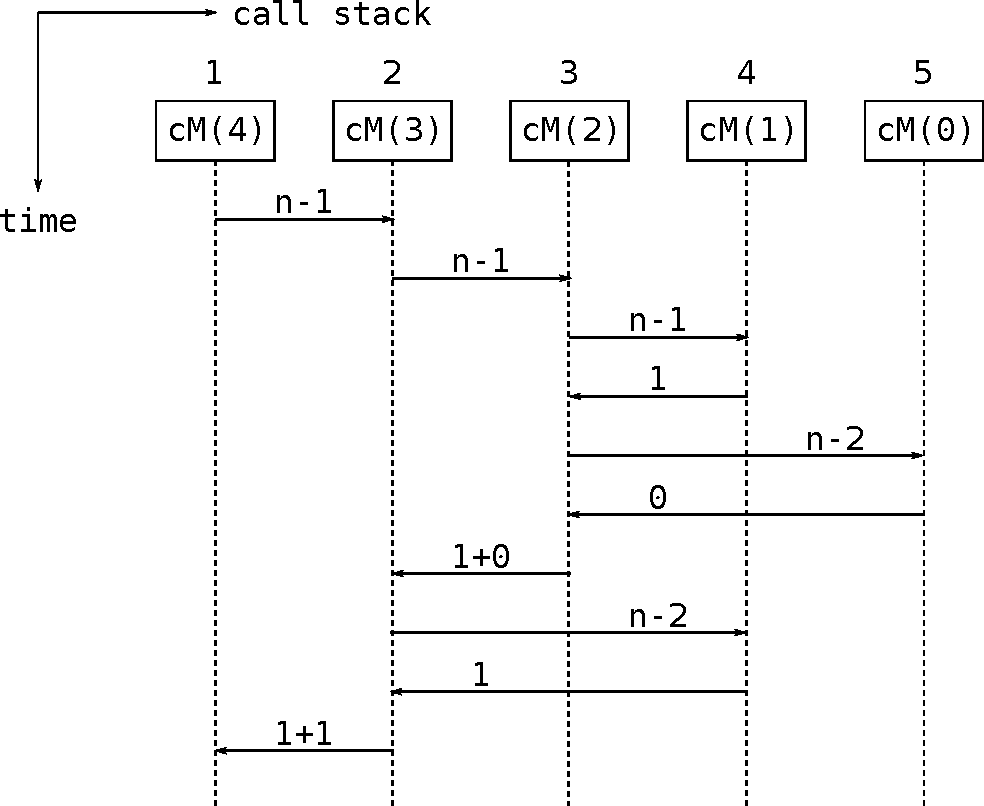
\includegraphics[width=0.6\textwidth]{callstack.pdf}
	\caption{Graphical explanation of call stack rising.}
	\label{pic:callstack}
\end{figure}

\newpage
\subsubsection*{Exercise 8}
\textit{Implement a recursive algorithm for the calculation of the
faculty (see presentation ALG2, page 9). Debug you method for the
faculty of 4.} \\

\lstinputlisting{../workspace/Snippets/src/faculty/Main.java}

\subsubsection*{Exercise 9}
\textit{Implement a recursive method to print an array forwards and
 backwards (see presentation ALG2, pages 29 and 30).} \\

\lstinputlisting{../workspace/Snippets/src/reverse/Main.java}

\subsubsection*{Exercise 10}
\textit{Implement a recursive method that is calculating the sum of
all integer values of an array. Make a documentation with javadoc.} \\

\lstinputlisting{../workspace/Snippets/src/sum/Main.java}

\subsubsection*{Additional Exercise}
\textit{Think about a algorithm that can perform a permutation on an array.
Lets say for the sequence 1,2,3,4.}

The idea is that we have to use a tree. The tree shows every possible path
that can be used for the rearrangement of the numbers. If we start with
the number 1, what are the possible paths that we can go trough? See the
graphical tree in picture \ref{pic:tree} to get an idea of it.

\begin{figure}[h!]
	\centering
	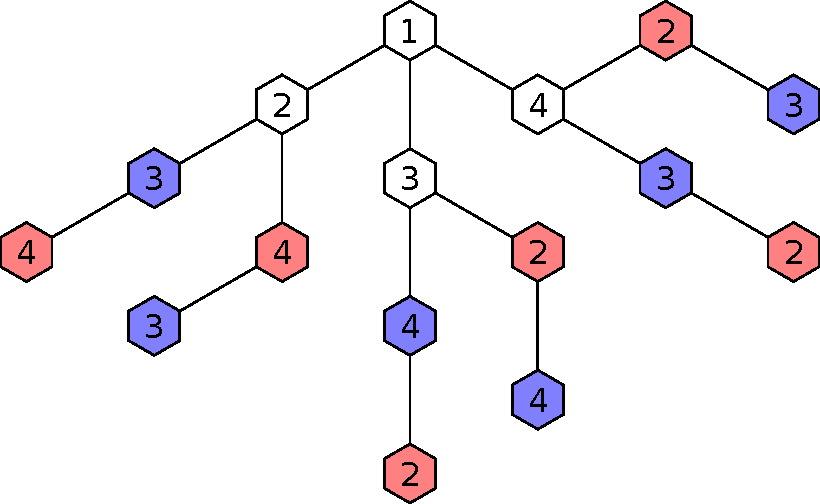
\includegraphics[width=0.5\textwidth]{tree.pdf}
	\caption{Tree for permutation of 1,2,3,4 beginning with 1.}
	\label{pic:tree}
\end{figure}

So we see, that the tricky part is at the end because the last two segments
are turned around while the other are just incremented.


\subsection{Team-Exercise}

\subsubsection{Exercise 1}
\textit{Solve the exercise 5.71} \\

\lstinputlisting{../workspace/StarWars/src/star/NameGenerator.java}
\lstinputlisting{../workspace/StarWars/src/star/Main.java}
